\documentclass[a4paper]{article}
%\usepackage{mathptmx}
\usepackage{amsmath}
\usepackage{amssymb}
\usepackage{amsthm}
\usepackage[retainorgcmds]{IEEEtrantools}
%\usepackage[square]{natbib}

% needs debian package texlive-math-extra
\usepackage{stmaryrd} % for \llbracket, \rrbracket (scott brackets)

\usepackage{tikz}
\usetikzlibrary{positioning}
\usetikzlibrary{matrix}

\newcommand{\arr}{\rightarrow}
\newcommand{\todo}[1]{\bigskip \noindent \emph{todo: #1}}
%\newcommand{\todo}[1]{}
\newcommand{\semantics}[1]{\llbracket #1 \rrbracket}

\newtheorem{defNuF}{Definition}[section]
\newtheorem{defNplaceSeparatedSum}[defNuF]{Definition}
\newtheorem{defF}[defNuF]{Definition}
\newtheorem{thmDomNuFisFixedPoint}[defNuF]{Proposition}
\newtheorem{defNuFCoalgebra}[defNuF]{Definition}
\newtheorem{obsNuFCoalgebraIsInjective}[defNuF]{Observation}
\newtheorem{defNuFCoalgebraPrime}[defNuF]{Definition}
\newtheorem{thmDomNuFisFinal}[defNuF]{Proposition}
\newtheorem{defSemantics}[defNuF]{Definition}
\newtheorem{lemSemanticAfterDeltaIsIdentity}[defNuF]{Lemma}
\newtheorem{lemSemanticAndFagreeOnOneStep}[defNuF]{Lemma}
\newtheorem{defStrictOrderNuF}[defNuF]{Definition}
\newtheorem{defPartialOrderNuF}[defNuF]{Definition}
\newtheorem{thmPONuFisPartial}[defNuF]{Proposition}
\newtheorem{thmPONuFisChainComplete}[defNuF]{Proposition}
\newtheorem{thmPONuFisADomain}[defNuF]{Proposition}
\newtheorem{defIMapsNuFToL}[defNuF]{Definition}
\newtheorem{thmIIsMonotone}[defNuF]{Proposition}
\newtheorem{thmIIsContinuous}[defNuF]{Proposition}

\begin{document}

\title{A Domain For The Natural Numbers With Computation Steps}
\author{Markus Klinik}
\maketitle

%\begin{abstract}
%Lorem ipsum.
%\end{abstract}

\section{What Are The Natural Numbers With Computation Steps?}

\section{What Is a Domain?}

\begin{itemize}

\item A domain is a CPO with a least element.

\item And what is a CPO?  A partial order where every chain has a least upper bound.

\item Finding a domain for the 1+X+X means finding a suitable CPO
together with a mapping from the 1+X+X to that CPO.

\item We then need to prove that the given construction is indeed a CPO with
least element.

\end{itemize}

\section{A Domain for 1+X+X}

\todo{We are currently on vacation in the land of CPOs and strict maps between them.
Or somesuch.}

\begin{defNplaceSeparatedSum}

The I-place separated sum functor is defined as follows.

\begin{equation}
\sum : \mathbf{Cpo}^I \arr \mathbf{Cpo} \nonumber
\end{equation}

\begin{equation}
\sum_{i \in I}{X_i} =
  \bigcup_{i \in I} \{ \langle i, a \rangle | a \in X_i \}
  \cup \{ \bot \} \nonumber
\end{equation}

\begin{equation}
\sum_{i \in I}{(f_i : X_i \arr Y_i)} :
  \sum_{i \in I}{X_i} \arr \sum_{i \in I}{Y_i} \nonumber
\end{equation}

\begin{equation*}
( \sum_{i \in I}f_i ) (x) = \left\{
  \begin{array}{rl}
     \langle i, f(a) \rangle & \text{if } x = \langle i, a \rangle
                               \text{ for some } i \in I \\
    \bot                     & \text{if } x = \bot
  \end{array} \right.
\end{equation*}

\end{defNplaceSeparatedSum}

That is, $\Sigma$ takes a family of sets to their disjoint union and adds a bottom
element to the result.  For a family of functions, it applies the corresponding
function to an element of the disjoint union.  We write $\kappa_i(a)$ for
$\langle i, a \rangle$.

\begin{defF}

The functor F is then defined as follows.

\begin{equation*}
FX = \sum{(1, X, X)}
\end{equation*}

\begin{equation*}
F(f : X \arr Y) = \sum{(\text{id}, f, f)}
\end{equation*}

Where $1 = \{*\}$ is the singleton CPO.

\end{defF}


\begin{defNuF}

Let $Z$ be the set of finite and infinite words generated by the following
grammar.

\begin{equation*}
Z ::= 0 \ |\ \bot \ |\ S Z \ |\ \_ Z
\end{equation*}

\end{defNuF}

Among those words are, for example, all Peano numbers like $0$, $S0$, $SS0$.
We also have arbitrary underscores mixed in between the successors: $\_0$,
$S\_S\_0$.  Instead of $0$, words can be terminated by $\bot$, e.g.  $S\bot$,
$S\_S\bot$.

Note that all finite words are finite sequences of $S$ and $\_$ which end with
either $0$ or $\bot$. All infinite words are $\omega$-sequences of $S$ and $\_$.

We write $|w|$ to denote the length of a word $w$.  The concatenation of two
words $w$, $v$ is denoted by their juxtaposition $wv$.  If $w$ or $v$ are
singleton words, we regard them sometimes as letters, sometimes as words, as the
situation requires.  The meaning should always be clear from the context.

\begin{thmDomNuFisFixedPoint}

The set $Z$ is a fixed point of the functor $F$.

\end{thmDomNuFisFixedPoint}

\begin{proof}

We need to show that $Z$ is isomorphic to $FZ$, that is, provide two functions
$\delta : Z \arr FZ$ and $\delta' : FZ \arr Z$ such that their composition is
the identity function, i.e.~$\delta \circ \delta' = \text{id}_{FZ}$ and $\delta'
\circ \delta = \text{id}_Z$.

\begin{defNuFCoalgebra}
Let $\delta : Z \arr FZ$ be defined as
  \begin{IEEEeqnarray}{rCl}
  \delta(\bot) & = & \bot \nonumber
  \\
  \delta(0) & = & \kappa_0(*) \nonumber
  \\
  \delta(Sw) & = & \kappa_1(w) \text{, for all } w \in Z  \nonumber
  \\
  \delta(\_w) & = & \kappa_2(w) \text{, for all } w \in Z  \nonumber
  \end{IEEEeqnarray}
\end{defNuFCoalgebra}

\begin{defNuFCoalgebraPrime}
Let $\delta' : FZ \arr Z$ be defined as
  \begin{IEEEeqnarray}{rCl}
  \delta'(\bot) & = & \bot \nonumber
  \\
  \delta'(\kappa_0(*)) & = & 0 \nonumber
  \\
  \delta'(\kappa_1(w)) & = & Sw \text{, for all } w \in Z  \nonumber
  \\
  \delta'(\kappa_2(w)) & = & \_w \text{, for all } w \in Z  \nonumber
  \end{IEEEeqnarray}
\end{defNuFCoalgebraPrime}

These equations hold.

\begin{IEEEeqnarray}{rCl}
\delta'(\delta(\bot)) & = & \delta'(\bot) = \bot \nonumber
\\
\delta'(\delta(0)) & = & \delta'(\kappa_0(*)) = 0 \nonumber
\\
\delta'(\delta(Sw)) & = & \delta'(\kappa_1(w)) = Sw \text{, for all } w \in Z \nonumber
\\
\delta'(\delta(\_w)) & = & \delta'(\kappa_2(w)) = \_w \text{, for all } w \in Z  \nonumber
\end{IEEEeqnarray}

\begin{IEEEeqnarray}{rCl}
\delta(\delta'(\bot)) & = & \delta(\bot) = \bot \nonumber
\\
\delta(\delta'(\kappa_0(*))) & = & \delta(0) = \kappa_0(*) \nonumber
\\
\delta(\delta'(\kappa_1(w))) & = & \delta(Sw)) = \kappa_1(w) \text{, for all } w \in Z  \nonumber
\\
\delta(\delta'(\kappa_2(w))) & = & \delta(\_w) = \kappa_2(w) \text{, for all } w \in Z  \nonumber
\end{IEEEeqnarray}

\end{proof}

\begin{obsNuFCoalgebraIsInjective}
$\delta$ is injective.
\end{obsNuFCoalgebraIsInjective}

\begin{thmDomNuFisFinal}
\label{thmDomNuFisFinal}

The set $Z$ is the largest fixed point for the functor $F$.

\end{thmDomNuFisFinal}

We need to show that any other fixed point of $F$ can be embedded into $Z$.  We
prove this by showing that $(Z, \delta)$ is a final coalgebra for $F$, that is,
for any other $F$-coalgebra $(C, \gamma : C \arr FC)$ there exists a unique
function $\semantics{-}_{\gamma} : C \arr Z$ such that
$F(\semantics{-}_{\gamma}) \circ \gamma = \delta \circ \semantics{-}_{\gamma}$,
i.e.~it makes the following diagram commute.

\begin{figure}[h]
\begin{center}
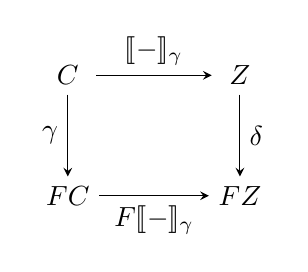
\begin{tikzpicture}
\matrix (m) [matrix of math nodes,row sep=3em,column sep=4em,minimum width=2em]
  {
     C & Z \\
     FC & FZ \\
  };
  \path[-stealth]
    (m-1-1) edge node [left] {$\gamma$} (m-2-1)
            edge node [above] {$\semantics{-}_{\gamma}$} (m-1-2)
    (m-2-1.east|-m-2-2) edge node [below] {$F\semantics{-}_{\gamma}$} (m-2-2)
    (m-1-2) edge node [right] {$\delta$} (m-2-2);
\end{tikzpicture}
\end{center}
\end{figure}

Before we prove this proposition, let's briefly reflect on what it would mean
for $(Z, \delta)$ to be the final coalgebra for $F$.

The idea behind the definitions of $Z$ and $\delta$ is that $Z$ has intrinsic
structure which resembles the structure of $F$.  We can regard $F$-coalgebras as
calculations that either diverge, terminate, or make one of two different
computation steps.  This is encoded as $\gamma(a)$ yielding $\bot$,
$\kappa_0(*)$, $\kappa_1(b)$ or $\kappa_2(b)$ respectively, where $a$ and $b$
are elements of $C$, which we regard as internal states of the computation. In
the latter two cases, the computation can continue from $b$, yielding another
one of the possible outcomes in the next step.

The set $Z$ has as elements finite and infinite words, where we can see one word
as the complete encoding of the behaviour of some $F$-coalgebra.  For example,
take $C = \{\bot, a\}$ and $\gamma(a) = \kappa_0(*)$, then the coalgebra $(C,
\gamma)$, has a very simple behaviour on $a$:  It terminates in the first step.
This behaviour is encoded in the singleton word $0$ in $Z$.

For another example, consider $C$ as above, but this time $\gamma(a) =
\kappa_1(a)$, i.e.~the computation makes one step and yields the state $a$
again.  From there, it continues with the same step, and so on, indefinitely.
This behaviour is represented in $Z$ by the infinite word of only Ss.

The function $\delta$ strips off the first letter of a word $w$, if possible,
and yields as result the rest of the word.  This corresponds to the behaviour of
$\gamma$ on some state $x$: $\gamma$ makes one step, and leaves us with the rest
of it's behaviour.  Our goal is to map $x$ to $w$ such that $\delta$ and
$\gamma$ coincide.

The intrinsic structure of $Z$ makes it possible to embed the states of other
$F$-coalgebras into $Z$. We map a state to the word which corresponds to the
state's behaviour.

\begin{defSemantics}

Let $(C, \gamma)$ be an $F$-coalgebra.  The function $\semantics{-}_{\gamma} : C
\arr Z$ is defined as follows.
\begin{IEEEeqnarray}{rCl}
\semantics{a}_{\gamma} & = & \text{ case } \gamma(a) \text{ of} \nonumber
\\
\bot_C & = & \bot_Z \nonumber
\\
\kappa_0(*) & = & 0 \nonumber
\\
\kappa_1(b) & = & S \semantics{b}_{\gamma} \nonumber
\\
\kappa_2(b) & = & \_ \semantics{b}_{\gamma} \nonumber
\end{IEEEeqnarray}

\end{defSemantics}

If it is clear from the context, we omit the subscript in
$\semantics{-}_{\gamma}$ and write $\semantics{-}$.


\begin{lemSemanticAfterDeltaIsIdentity}
\label{lemSemanticAfterDeltaIsIdentity}

$\semantics{-}_{F\delta} \circ \delta = \text{id}_{\delta}$

\end{lemSemanticAfterDeltaIsIdentity}

\begin{proof}
Admitted.
\end{proof}


\begin{lemSemanticAndFagreeOnOneStep}
\label{lemSemanticAndFagreeOnOneStep}

Let $(C, \gamma)$ be an $F$-coalgebra. For all $a$ in $C$ and $w$ in $\{S,
\_\}^*$:

\begin{itemize}
\item
  if $\gamma(a) = \kappa_1(b)$ then $\delta(w\semantics{a}) = \delta(wS
  \semantics{b})$ and $\delta(wf(a)) = \delta(wSf(b))$
\item
  if $\gamma(a) = \kappa_2(b)$ then $\delta(w\semantics{a}) =
  \delta(w\_\semantics{b})$ and $\delta(wf(a)) = \delta(w\_f(b))$
\end{itemize}

\end{lemSemanticAndFagreeOnOneStep}

\begin{proof}
Admitted.
\end{proof}


The informal idea that $(Z, \delta)$ encodes all possible behaviours of
$F$-coalgebras is made explicit in the following proof of proposition
\ref{thmDomNuFisFinal}.

\begin{proof}{(Proposition \ref{thmDomNuFisFinal})}

We need to prove two things.

  \begin{enumerate}
  \item
    The function $\semantics{-}$ is an $F$-coalgebra homomorphism.
  \item
    The function $\semantics{-}$ is unique, i.e.~any other $F$-coalgebra
    homomorphism $f : C \arr Z$ agrees with $\semantics{-}$ on every element of C.
  \end{enumerate}

1. For $\semantics{-}$ to be an
$F$-coalgebra homomorphism, it has to satisfy the equation $\delta \circ
\semantics{-} = F\semantics{-} \circ \gamma$.  Let $a$ be an element of $C$. We
proceed by case distinction on $\gamma(a)$.

Case $\gamma(a) = \bot$:
\begin{equation*}
\delta(\semantics{a}) = \delta(\bot) = \bot =
F\semantics{\bot} = F\semantics{\gamma(a)}
\end{equation*}

Case $\gamma(a) = \kappa_0(*)$:
\begin{equation*}
\delta(\semantics{a}) = \delta(0) = \kappa_0(*)
= \kappa_0(\text{id}(*)) = F\semantics{\kappa_0(*)} = F\semantics{\gamma(a)}
\end{equation*}

Case $\gamma(a) = \kappa_1(b)$:
\begin{equation*}
\delta(\semantics{a}) = \delta(S \semantics{b}) = \kappa_1(\semantics{b}) =
F\semantics{\kappa_1(b)} = F\semantics{\gamma(a)}
\end{equation*}

Case $\gamma(a) = \kappa_2(b)$:
\begin{equation*}
\delta(\semantics{a}) = \delta(\_ \semantics{b}) = \kappa_2(\semantics{b}) =
F\semantics{\kappa_2(b)} = F\semantics{\gamma(a)}
\end{equation*}

2. Assume $f : C \arr Z$ is another $F$-coalgebra homomorphism, that is, it
satisfies the equation $\delta \circ f = Ff \circ \gamma$.  We proceed by
constructing a bisimulation relation between $\delta \circ f$ and $\delta \circ
\semantics{-}$.  Let

\begin{equation*}
R \subseteq FZ \times FZ =
  \{ \langle \delta(wf(a)) , \delta(w\semantics{a}) \rangle
   \ |\  a \in C, w \in \{ S, \_ \}^*
  \}
\end{equation*}

\todo{Use lemmas \ref{lemSemanticAfterDeltaIsIdentity} and
\ref{lemSemanticAndFagreeOnOneStep} to prove that R is a bisimulation relation.}

For $w = \epsilon$, we have that $\langle \delta(f(a)) , \delta(\semantics{a})
\rangle$ is in $R$ for all $a$ in $C$.  This gives us the equality $\delta \circ
f = \delta \circ \semantics{-}$, from which, by injectivity of $\delta$, we
infer $f = \semantics{-}$.


\end{proof}

\begin{defStrictOrderNuF}

Let the relation $\sqsubset$ on $Z \times Z$ be defined as: two
words $s$ and $t$ are in relation $s \sqsubset t$ iff $s$ is finite and $|s|
\leq |t|$ and $s_{|s|-1} = \bot$ and for all $i < |s|-1: s_i = t_i$.

\end{defStrictOrderNuF}


\begin{defPartialOrderNuF}

Let $\sqsubseteq$ be the reflexive closure of $\sqsubset$.

\end{defPartialOrderNuF}


\begin{figure}
\begin{center}
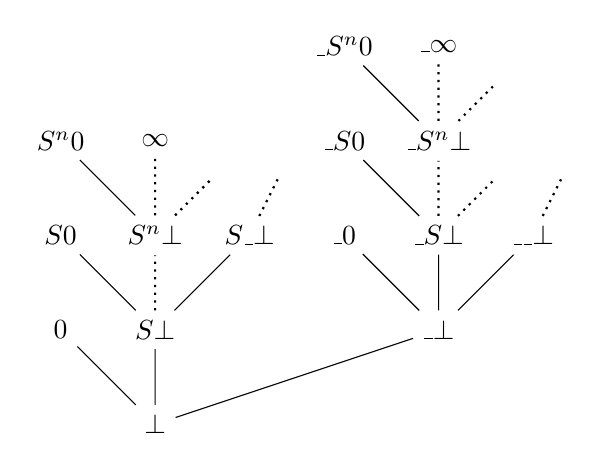
\begin{tikzpicture}
 [ grow'=up
 , scale=1.2
 , level distance=1cm
 , level 1/.style={sibling distance=3cm}
 , level 2/.style={sibling distance=1cm}
 , normal/.style={thin, solid}
 , skipping/.style={thick, dotted}
 , and so on/.style={thick, dotted, sibling distance=0.6cm, level distance=0.6cm}
 ]
  \node {$\bot$}
    child [sibling distance=1cm] { node {$0$} }
    child
    {
      node {$S\bot$}
      child { node {$S0$} }
      child [skipping]
      {
        %node {$SS\bot$}
        %child { node {$SS0$} }
        %child [skipping]
        %{
          node {$S^n\bot$}
          child [normal] { node {$S^n0$} }
          child [skipping] { node {$\infty$} }
          child [and so on] {}
        %}
        %child [and so on] {}
      }
      child
      {
        node {$S\_\bot$}
        child [missing] {}
        child [and so on] {}
      }
    }
    child
    {
      node {$\_ \bot$}
      child { node {$\_0$} }
      child
      {
        node {$\_S\bot$}
        child { node {$\_S0$} }
        child [skipping]
        {
          node {$\_S^n\bot$}
          child [normal] { node {$\_S^n0$} }
          child { node {$\_\infty$} }
          child [and so on] {}
        }
        child [and so on] {}
      }
      child
      {
        node {$\_\_\bot$}
        child [missing] {}
        %child [missing] {}
        child [and so on] {}
      }
    }
  ;
\end{tikzpicture}
\end{center}
\caption{The domain $(Z, \sqsubseteq)$.}
\label{fig:DomainOfNuF}
\end{figure}

The definition of $\sqsubseteq$ is intended to define an information ordering on
$Z$.  Its relation graph is shown in figure \ref{fig:DomainOfNuF}.
Informally speaking, nodes closer to the root of the tree give less information
than nodes further up the tree.  Consider a process that step-by-step calculates
an element of $Z$.  We want to interpret the result of the computation
based on the output we have seen so far.  The root node can then be read as ``it
could be any number''.  The value $S\bot$ can be read as ``it is at least one''.
Any value that ends with a $0$ tells us a concrete number, together with the
fact that the process has terminated.  As with flat domains, concrete values are
incomparable, so we don't distinguish between $1$ and $2$ from the viewpoint of
information ordering.

When looking at the subtree of $\_\bot$, we see that its structure is similar
to the whole domain itself, except that every value is prefixed with one additional
underscore.  Nodes in this subtree can be interpreted similarly as described
above, only that it took the process one internal computation step more to
get to this point.

\todo{What's with the sequence of infinite underscores, or a finite number of
sucessors followed by an infinite number of underscores?  Do we regard them as
infinity?}

\todo{Are the two infinities in the picture the same?}

\begin{thmPONuFisPartial}

The relation $\sqsubseteq$ is a partial order.

\end{thmPONuFisPartial}


\begin{proof}

We have to prove the that $\sqsubseteq$ is reflexive, transitive, and
antisymmetric.

Reflexive: by definition.

Transitive: We have to prove that if $s \sqsubseteq t$ and $t \sqsubseteq u$
then $s \sqsubseteq u$ for all words $s$, $t$, $u$. We do so by distinguishing
four cases.

1. If $s = t = u$ then $s \sqsubseteq u$ follows from reflexivity.

2, 3. The cases $s \neq t \wedge t = u \wedge s \sqsubseteq t$ and $s = t
\wedge t \neq u \wedge t \sqsubseteq u$ are trivial.

4. $s \neq t \wedge t \neq u \wedge s \sqsubseteq t \wedge t \sqsubseteq u$ We
have: $|s| \leq |t| \leq |u|$ and $s_{|s|-1} = \bot$ and $t_{|t|-1} = \bot$ and
for all $i < |s|-1: s_i = t_i$ and for all $j < |t|-1: t_j = u_j$.  But this
means, because of $|s| \leq |t|$: for all $i < |s|-1: s_i = u_i$, hence $s
\sqsubseteq u$.

Antisymmetric: We have to prove that if $s \sqsubseteq t \wedge t \sqsubseteq
s$ then $s = t$.  The premise is either the case because $s = t$ to begin with,
or we have: $s$ is finite and $|s| \leq |t|$ and $s_{|s|-1} = \bot$ and for all $j <
i: s_j = t_j$ and $t$ is finite and $|t| \leq |s|$ and $t_{|t|-1} = \bot$ and for all
$j < i: t_j = s_j$.  But then $s$ and $t$ are both finite, of the same length,
and agree in all elements, hence $s = t$.

\end{proof}

\begin{thmPONuFisChainComplete}

The relation $\sqsubseteq$ is chain complete.

\end{thmPONuFisChainComplete}

We need to show that every $\omega$-chain in $Z$ has a least upper bound.
An $\omega$-chain in $Z$ is a sequence $f : \mathbb{N} \arr Z$ such
that for all $i \in \mathbb{N}: f(i) \sqsubseteq f(i + 1)$.


\begin{thmPONuFisADomain}

The structure $(Z, \sqsubseteq)$ is a domain.

\end{thmPONuFisADomain}

We need to show that $(Z, \sqsubseteq)$ has a least element, i.e.~there is
an element $s \in Z$ such that for any other element $t \in Z s
\sqsubseteq t$.

Next, we want to check if we can recover the lazy natural numbers, denoted by
$L$, from the 1+X+X by giving a continuous map between $Z$ and $L$.
The domain $(L, \sqsubseteq)$ is given informally in figure
\ref{fig:DomainOfLazyNaturals}.

%\begin{figure}
%\begin{center}
%\begin{tikzpicture}
  %\node {$\underline 0$} [grow'=up, sibling distance=4.0em, level distance=1.8em]
    %child { node {$0$} }
    %child
    %{
      %node {$\underline 1$}
      %child { node {$1$} }
      %child
      %{
        %node {$\underline 2$}
        %child { node {$2$} }
        %child [thick, dotted]
        %{
          %node {$\underline n$}
          %child [thin, solid] { node {$n$} }
          %child { node {$\infty$} }
        %}
      %}
    %}
  %;
%\end{tikzpicture}
%\end{center}
%\caption{The domain of the lazy natural numbers.}
%\label{fig:DomainOfLazyNaturals}
%\end{figure}

\begin{figure}
\begin{center}
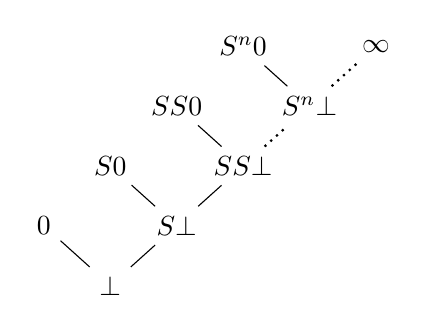
\begin{tikzpicture}[scale=1.2]
  \node {$\bot$} [grow'=up, sibling distance=4.0em, level distance=1.8em]
    child { node {$0$} }
    child
    {
      node {$S\bot$}
      child { node {$S0$} }
      child
      {
        node {$SS\bot$}
        child { node {$SS0$} }
        child [thick, dotted]
        {
          node {$S^n\bot$}
          child [thin, solid] { node {$S^n0$} }
          child { node {$\infty$} }
        }
      }
    }
  ;
\end{tikzpicture}
\end{center}
\caption{The domain of the lazy natural numbers.}
\label{fig:DomainOfLazyNaturals}
\end{figure}

\begin{defIMapsNuFToL}

Define the function $I : Z \arr L$ as follows: \ldots

\end{defIMapsNuFToL}


\begin{thmIIsMonotone}

The function $I$ is monotone.

\end{thmIIsMonotone}


\begin{thmIIsContinuous}

The function $I$ is continuous.

\end{thmIIsContinuous}

\section{Further directions}

\begin{itemize}
\item Embed 1+X+X into some coinductive PCF.
\item Analyze if the domain composes nicely (or at all) with the other
denotations.
\item Can we generalize the construction of the domain to arbitrary
F-coalgebras?
\end{itemize}

\section{Bibliographic notes}

Lorem ipsum \cite{Pierce1991} \cite{Gunter1992} \cite{Bird1997}
\cite{Mitchell1996} \cite{Allison1986} \cite{Capretta2002}

\todo{Barr and Wells "Cats for CompSci", Escardo "On lazy nats"}

\bibliographystyle{plain}
\bibliography{computer_science}
\end{document}

% vim: textwidth=80
